% This is a LaTeX thesis template for Adam Mickiewicz University.
% to be used with Rmarkdown
% This template was produced by Jakub Nowosad
% Version: 16 February 2020

% Inspired by:
% This is a LaTeX thesis template for Monash University.
% to be used with Rmarkdown
% This template was produced by Rob Hyndman
% Version: 6 September 2016

\documentclass{amuthesis}
% \usepackage[polish]{babel}
\usepackage{polski}
\renewcommand{\figurename}{Rycina} % Redefine default figure caption %
\renewcommand{\tablename}{Tabela} % Redefine default table caption %
%%%%%%%%%%%%%%%%%%%%%%%%%%%%%%%%%%%%%%%%%%%%%%%%%%%%%%%%%%%%%%%
% Add any LaTeX packages and other preamble here if required
%%%%%%%%%%%%%%%%%%%%%%%%%%%%%%%%%%%%%%%%%%%%%%%%%%%%%%%%%%%%%%%
\usepackage{booktabs,tabularx} % Allows kableExtra to work %
\usepackage{indentfirst} % Adds indent in the first paragraph %
\usepackage{bookmark} % Adds indent in the first paragraph %

\author{Tomasz Matuszek}
\title{Ocena wpływu zastosowania kanału termalnego Landsat na wyniki
nadzorowanej klasyfikacji pokrycia terenu}
\def\titleeng{Measuring impact of adding Landsat 8 thermal band on
supervised land cover classification}
\def\degreetitle{Praca inżynierska}
\def\major{Geoinformacja}
\def\albumid{000000}
\def\thesisyear{2022}
% Add subject and keywords below
\hypersetup{
     %pdfsubject={The Subject},
     %pdfkeywords={Some Keywords},
     pdfauthor={Tomasz Matuszek},
     pdftitle={Ocena wpływu zastosowania kanału termalnego Landsat na
wyniki nadzorowanej klasyfikacji pokrycia terenu},
     pdfproducer={quarto with LaTeX}
}

\bibliography{thesis,packages}

\begin{document}

\pagenumbering{arabic}

\titlepage

\bookmarksetup{startatroot}

\hypertarget{streszczenie}{%
\chapter*{Streszczenie}\label{streszczenie}}
\addcontentsline{toc}{chapter}{Streszczenie}

\textbf{Abstrakt}

Streszczenie powinno przedstawiać skrótowo główny problem pracy i jego
rozwiązanie. Możliwa struktura streszczenia to: (1) 1-3 zdania wstępu do
problemu (czym się zajmujemy, dlaczego jest to ważne, jakie są
problemy/luki do wypełnienia), (2) 1 zdanie opisujące cel pracy, (3) 1-3
zdania przedstawiające użyte materiały (dane) i metody (techniki,
narzędzia), (4) 1-3 zdania obrazujące główne wyniki pracy, (5) 1-2
zdania podsumowujące; możliwe jest też określenie dalszych
kroków/planów.

Słowa kluczowe: (4-6 słów/zwrotów opisujących treść pracy, które nie
wystąpiły w tytule)

\textbf{Abstract}

The abstract must be consistent with the above text.

Keywords: (as stated before)

\newpage

\setstretch{1.2}\sf\tighttoc\doublespacing

\bookmarksetup{startatroot}

\hypertarget{sec-wprowadzenie}{%
\chapter{Wprowadzenie}\label{sec-wprowadzenie}}

\begin{itemize}
\item
  zastosowania i istotność map pokrycia terenu
\item
  uczenie maszynowe i klasyfikacja nadzorowana obrazów satelitarnych
  jako narzędzie do tworzenia map pokrycia terenu
\item
  zwrócenie uwagi na częste pomijanie kanału termalnego w modelach
  klasyfikacyjnych, nie do końca jasny wpływ informacji termalnej na
  wyniki klasyfikacji
\item
  celem pracy jest stworzenie mapy pokrycia terenu metropolii
  poznańskiej oraz ocena wpływu kanału termalnego na wyniki modelu
\end{itemize}

\begin{center}\rule{0.5\linewidth}{0.5pt}\end{center}

Wprowadzenie powinno mieć charakter opisu od ogółu do szczegółu (np.
trzy-pięć paragrafów). Pierwszy paragraf powinien być najbardziej
ogólny, a kolejne powinny przybliżać czytelnika do problemu.
Przedostatni paragraf powinien określić jaki jest problem (są problemy),
który praca ma rozwiązać i dlaczego jest to (są one) ważne.

Wprowadzenie powinno być zakończone stwierdzeniem celu pracy. Dodatkowo
tutaj może znaleźć się również krótki opis co zostało zrealizowane w
pracy.

\bookmarksetup{startatroot}

\hypertarget{sec-lit}{%
\chapter{Przegląd literatury}\label{sec-lit}}

\begin{center}\rule{0.5\linewidth}{0.5pt}\end{center}

Ten rozdział zawiera wyjaśnienie kontekstu pracy.

Pisząc ten rozdział proszę pomyśleć o osobach, które zupełnie nie znają
opisywanej tematyki. Należy tutaj krok po kroku wyjaśnić podstawowe
koncepcje, istotność problemu, wyniki poprzednich podobnych badań, itd.
Ten rozdział obejmuje tylko kwestie, które już zostały wykonane przez
inne osoby - nowe wyniki mają swoje miejsce w rozdziale
\ref{sec-wyniki}.

Każda kwestia opisana w tym rozdziale powinna być cytowana. Dodatnie
cytowania odbywa się poprzez uzupełnienie pliku \texttt{thesis.bib}
zapisem w formacie BibTeX, a następnie dodanie nazwy referencji
poprzedzonej znakiem \texttt{@}. Przykładowo, zacytowanie książki
Geocomputation with R odbywa się poprzez
\autocite{lovelace_geocomputation_2019}.

W przypadku, gdy cytowanie zostało poprawnie wpisane oraz istnieje w
pliku \texttt{thesis.bib} to bibliografia powinna się automatycznie
wygenerować na końcu pracy.

W przypadku, gdy praca dyplomowa opisuje konkretny obszar to można po
tym rozdziale stworzyć kolejny rozdział opisujący ``obszar badań''.

Ten i kolejne rozdziału moją mieć także podrozdziały. Tworzenie
podrozdziałów polega na stworzeniu nowej linii rozpoczynającej się od
znaków \texttt{\#\#} a następnie tytułu podrozdziału. Dodatkowo w
postaci \texttt{\{\#sec-\}} można dodać skrót nazwy
rozdziału/podrozdziału umożliwiający odnoszenie się do niego używając
operatora \texttt{{[}-@sec{]}}.

\bookmarksetup{startatroot}

\hypertarget{sec-dane}{%
\chapter{Dane źródłowe}\label{sec-dane}}

Do przeprowadzenia analiz wykorzystano dwa typy danych:

\begin{itemize}
\item
  rastrowe dane satelitarne Landsat pobrane przy pomocy narzędzia GLAD
  ARD
\item
  punktowe dane o pokryciu terenu pozyskane w wyniku programu LUCAS
\end{itemize}

\hypertarget{sec-sat}{%
\section{Dane satelitarne}\label{sec-sat}}

\begin{itemize}
\item
  opis procesu obróbki danych Landsat wykonany przez zespół z
  Uniwersytetu Maryland
\item
  proces pobierania danych
\item
  struktura danych GLAD ARD
\end{itemize}

\hypertarget{sec-landcover}{%
\section{Dane o pokryciu terenu}\label{sec-landcover}}

\begin{itemize}
\item
  czym jest program LUCAS i jak powstają dane w ramach jego działania
\item
  LUCAS Grid i LUCAS Micro Data
\item
  struktura danych punktowych, opis dodatkowych kolumn poza kategorią
  pokrycia terenu
\item
  obróbka danych w celu wybrania odpowiednych punktów treningowych i
  reklasyfikacji do wspólnego podziału na kategorie pokrycia terenu
\end{itemize}

\begin{center}\rule{0.5\linewidth}{0.5pt}\end{center}

Celem tego rozdziału jest przedstawienie użytych w pracy danych. Należy
wyjaśnić jakie dane zostały użyte, jakiego są one rodzaju, dla jakiego
okresu zostały pobrane/stworzone, co one zawierają, etc.

W tym rozdziale warto dodać ryciny i tabele przedstawiające użyte dane.

Zwróć uwagę, że poniższe bloki kodu mają parametr
\texttt{\#\textbar{}\ echo:\ false}; oznacza to, że będą one niewidoczne
w wynikowym pliku PDF. Każdy z bloków kodu musi mieć unikalną nazwę; w
przypadku rycin powinna się~ona rozpoczynać od prefiksu \texttt{fig-}.
Dodanie podpisu pod rycinę odbywa się używając parametru
\texttt{\#\textbar{}\ fig-cap:}. Następnie do tej ryciny można się
odnieść używając operatora \texttt{{[}-@{]}}.

Podobnie wygląda odnoszenie się do plików graficznych. Tutaj wewnątrz
bloku kodu należy użyć funkcji \texttt{knitr::include\_graphics()}
(Rycina \ref{fig-rycina2}). Dodatkowo możliwa jest zmiana rozmiary
obrazka używając parametrów takich jak \texttt{\#\textbar{}\ out-width:}
i \texttt{\#\textbar{}\ out-height:}.

\begin{figure}[t]

{\centering 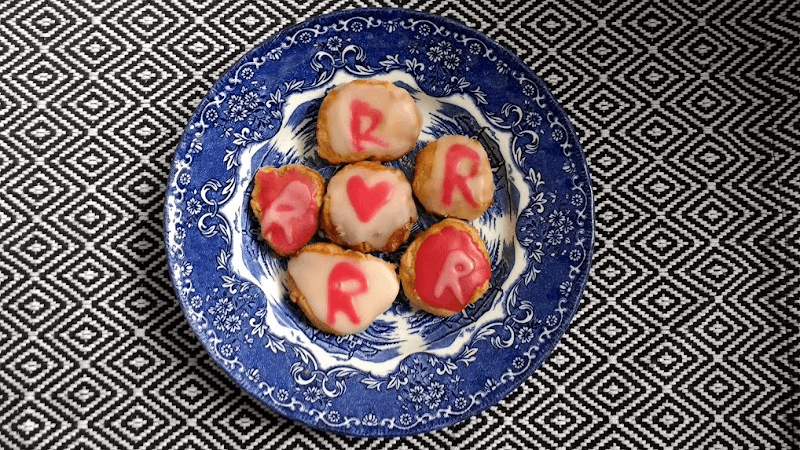
\includegraphics[width=1\textwidth,height=3.125in]{./figures/rcookies.png}

}

\caption{\label{fig-rycina2}Moja druga rycina}

\end{figure}

Odnoszenie się do tabel odbywa się poprzez operator \texttt{{[}-@{]}}
wraz z prefiksem \texttt{tbl-}. Natomiast tworzenie podpisu nad tabelą
ma miejsce używając parametru \texttt{\#\textbar{}\ tbl-cap:}. Dodatkowo
możliwe jest użycie pakietu \textbf{kableExtra} \autocite{R-kableExtra}
do określenia szerokości kolumn (Tabela \ref{tbl-tabela1}).

\hypertarget{tbl-tabela1}{}
\begin{table}
\caption{\label{tbl-tabela1}Moja pierwsza tabela }\tabularnewline

\centering
\begin{tabular}{>{\raggedleft\arraybackslash}p{2cm}>{\raggedright\arraybackslash}p{4cm}}
\toprule
a & b\\
\midrule
1 & a\\
2 & b\\
3 & c\\
4 & d\\
5 & e\\
\bottomrule
\end{tabular}
\end{table}

\bookmarksetup{startatroot}

\hypertarget{sec-metody}{%
\chapter{Metody}\label{sec-metody}}

\hypertarget{sec-r}{%
\section{Środowisko języka R}\label{sec-r}}

Krótki opis języka R oraz RStudio. Wymienienie wykorzystanych
pakietów/bibliotek.

\hypertarget{sec-ml}{%
\section{Metody uczenia maszynowego}\label{sec-ml}}

\begin{itemize}
\item
  czym jest uczenie maszynowe i do czego się je wykorzystuje
\item
  klasyfikacja a regresja
\item
  klasyfikacja nadzorowana a nienadzorowana
\end{itemize}

\hypertarget{sec-rf}{%
\subsection{\texorpdfstring{Algorytm lasów losowych (ang.\emph{random
forest})}{Algorytm lasów losowych (ang.random forest)}}\label{sec-rf}}

\begin{itemize}
\item
  czym jest drzewo decyzyjne
\item
  jak działają lasy losowe
\end{itemize}

\hypertarget{sec-resampling}{%
\subsection{Metody oceny jakości modelu}\label{sec-resampling}}

\begin{itemize}
\item
  idea resamplingu
\item
  miary jakości modelu klasyfikacyjnego
\end{itemize}

\hypertarget{sec-tuning}{%
\subsection{Tuning parametrów modelu}\label{sec-tuning}}

\begin{itemize}
\item
  czym jest tuning parametrów?
\item
  resampling zagnieżdżony
\end{itemize}

\begin{center}\rule{0.5\linewidth}{0.5pt}\end{center}

Rozdział \textbf{Metody} zawiera opis użytych metod (np. statystycznych
czy geostatystycznych) oraz technologii (np. pakiety R). Opis każdej z
metod czy technologi powinien być zwarty i zawierać tylko najważniejsze
informacje z punktu widzenia pracy dyplomowej.

Każda użyta metoda i technologia powinna być zacytowana. W przypadku
pakietów R, wystarczy wypełnić poniższy blok kodu (zwróć uwagę, że ten
blok kodu ma parametr \texttt{echo:\ false}; oznacza to, że będzie on
niewidoczny w wynikowym pliku PDF)\ldots{}

\ldots{} a następnie zacytować pakiet używając znaku \texttt{@}, po
którym podać nazwę pakietu rozpoczynającą się od prefiksu \texttt{R-}.
Przykładowe cytowanie języka R bez nawiasu to \textcite{R-base}, a
pakietu \textbf{kableExtra} w nawiasie to \autocite{R-kableExtra}.
Więcej przykładów cytowania można znaleźć na stronie
https://rmarkdown.rstudio.com/authoring\_bibliographies\_and\_citations.html\#citations.

W przypadkach, gdy cytowanie istnieje, ale nie jest pakietem R to należy
dodać je do pliku \texttt{thesis.bib} i użyć powyższej składni ze
znakiem \texttt{@}. W ostateczności, gdy dana technologia nie posiada
cytowania, należy podać jej adres internetowy.

\bookmarksetup{startatroot}

\hypertarget{sec-wyniki}{%
\chapter{Wyniki}\label{sec-wyniki}}

\hypertarget{sec-mapa}{%
\section{Wynikowa mapa pokrycia terenu}\label{sec-mapa}}

\begin{itemize}
\item
  mapa pokrycia terenu aglomeracji poznańskiej
\item
  mapa prawdopodobieństwa/pewności wybrania danej klasy
\end{itemize}

\hypertarget{sec-ocena}{%
\section{Ocena jakości modelu klasyfikacyjnego}\label{sec-ocena}}

Tabela ze wskaźnikami:

\begin{itemize}
\item
  skuteczność (OA)
\item
  błąd klasyfikacji (CE)
\item
  skuteczność producenta i użytkownika (PA, UA)
\item
  współczynnik Kappa
\end{itemize}

\hypertarget{sec-wplyw}{%
\section{Ocena wpływu kanału termalnego na wyniki
klasyfikacji}\label{sec-wplyw}}

\begin{itemize}
\item
  porównanie wskaźników z i bez kanału termalnego
\item
  średnia temperatura dla każdej klasy pokrycia terenu
\item
  wykresy uśredniające wpływ zmiennych na model, profile zmiennych
\item
  mapa wpływu kanału termalnego na model (metoda agregacji rastra oraz
  interpolacji z punktów LUCAS)
\item
  średni wpływ kanału termalnego na każdą klasę pokrycia terenu
\item
  mapa różnic pomiędzy modele pokrycia terenu z i bez kanału termalnego,
  macierz zmian
\end{itemize}

\begin{center}\rule{0.5\linewidth}{0.5pt}\end{center}

Część \textbf{Wyniki} może składać się z jednego lub więcej rozdziałów.
Każdy z tych rozdziałów powinien mieć tytuł adekwatny do swojej treści.

Rozdziały wynikowe powinny korzystać z wiedzy opisanej w poprzednich
rozdziałach (Rozdziały \ref{sec-lit}, \ref{sec-dane}, \ref{sec-metody}).
W przypadku prac analitycznych, ich treść powinna przedstawiać kolejne
etapy eksploracji i analizy danych. W przypadku prac technicznych, treść
tych rozdziałów powinna opisywać stworzone narzędzia, a następnie
pokazywać ich zastosowanie/a.

W przypadku prac technicznych warto pokazywać fragmenty napisanego
rozwiązania lub jego wywołania używając bloków kodu.

\begin{Shaded}
\begin{Highlighting}[]
\NormalTok{moja\_funkcja }\OtherTok{=} \ControlFlowTok{function}\NormalTok{(x)\{}
  \FunctionTok{cat}\NormalTok{(x, }\StringTok{"rządzi!"}\NormalTok{)}
\NormalTok{\}}
\FunctionTok{moja\_funkcja}\NormalTok{(}\StringTok{"Autor tej pracy"}\NormalTok{)}
\end{Highlighting}
\end{Shaded}

\begin{verbatim}
Autor tej pracy rządzi!
\end{verbatim}

\bookmarksetup{startatroot}

\hypertarget{podsumowanie}{%
\chapter{Podsumowanie}\label{podsumowanie}}

\begin{center}\rule{0.5\linewidth}{0.5pt}\end{center}

Podsumowanie pracy jest w pewnym sensie znacznie rozbudowanym
abstraktem. Należy wyliczyć i opisać osiągnięcia uzyskane w pracy
dyplomowej. Tutaj jednak (w przeciwieństwie do np. rozdziału
\ref{sec-wprowadzenie}) należy przechodzić od szczegółu do ogółu - co
zostało stworzone/określone, jak zostało to zrobione, jakie ma to
konsekwencje, itd.

Ten rozdział powinien też zawierać opis kwestii, których nie udało się
rozwiązać w pracy dyplomowej (i dlaczego się nie udało) oraz pomysły na
przyszłe ulepszenie uzyskanych wyników lub dalsze badania.

\printbibliography[heading=bibintoc, title=Bibliografia]

\end{document}
